

\renewcommand{\EntradaBibtex}{MarcoNuno_Revista_2023_09_00}

\begin{frame}{\citetitle{\EntradaBibtex}$^*$ (1)}
\begin{block}{Motivación} 
Tamaulipas es uno de los principales productores de cítricos. Mucho de la separación de la producción se hace aún de manera manual
\end{block} 
Se propone un sistema de alto desempeño para separar los citricos en una banda transportadora.
\begin{itemize}
\item Se utilizó un FPGA (Spartan6 Industrial Video Processing Kit) y el lenguaje de programación VHDL
\item La cámara está ubicada en un compartimiendo con luz controlada
\item Se efectúa la separación por tamaño y por nivel de madurez
\end{itemize}
\footfullcite*{\EntradaBibtex}
\end{frame}


\begin{frame}{\citetitle{\EntradaBibtex} (2)}
%\begin{block}{Pantallas Principales} 
\begin{center}
	\begin{tabular}{ccc}
		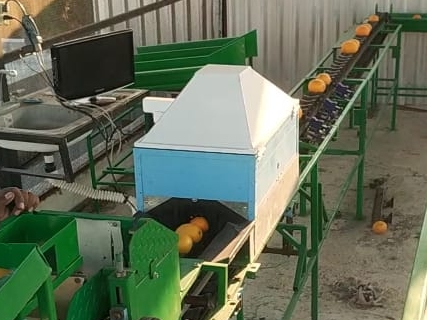
\includegraphics[width=0.25\linewidth]{2023_ConteoNaranjasBandaTransportadora/figs/ImagenBanda.png} &
		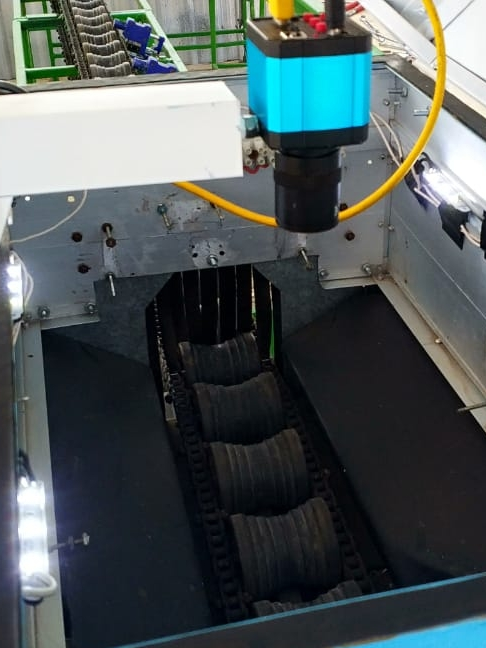
\includegraphics[width=0.25\linewidth]{2023_ConteoNaranjasBandaTransportadora/figs/interior.png} &
		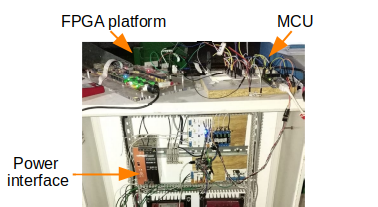
\includegraphics[width=0.45\linewidth]{2023_ConteoNaranjasBandaTransportadora/figs/ImagenTablero.png} \\
	\end{tabular}
\end{center}
\end{frame}


\begin{frame}{\citetitle{\EntradaBibtex} (3)}
%\begin{block}{Pantallas Principales} 
\begin{center}
	\begin{tabular}{c}
		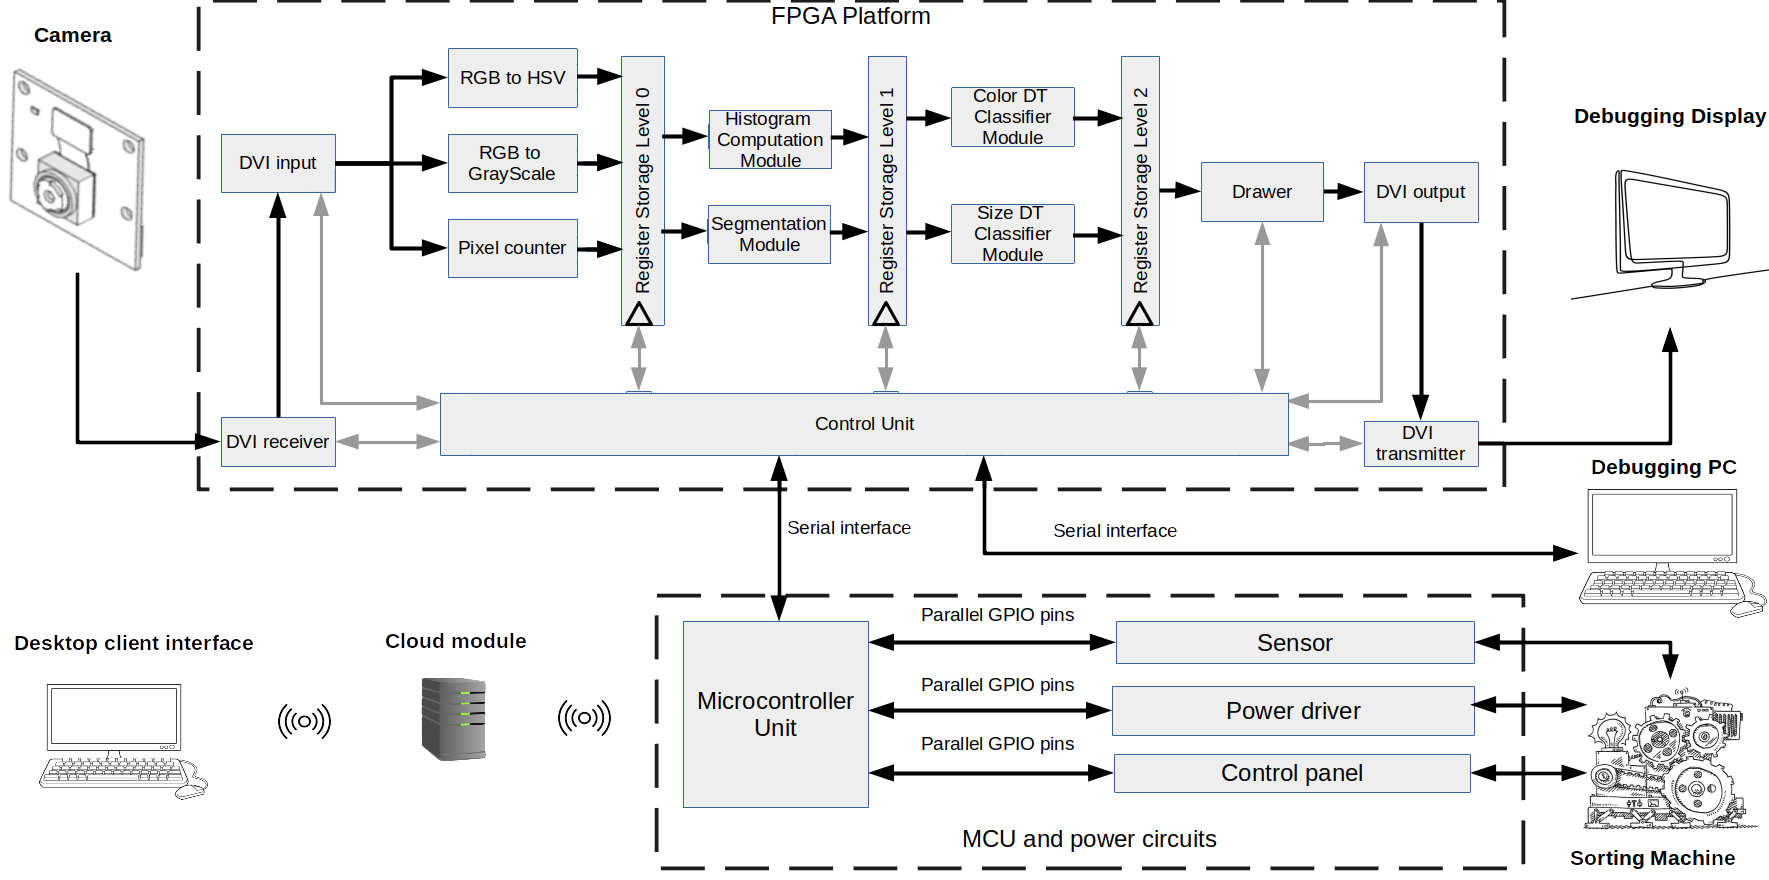
\includegraphics[width=0.65\linewidth]{2023_ConteoNaranjasBandaTransportadora/figs/Figura_ArticuloAntonio_MainSystem_VersionESL.png} \\
	\end{tabular}
\end{center}
\end{frame}



\begin{frame}{\citetitle{\EntradaBibtex} (4)}
%\begin{block}{Pantallas Principales} 
\begin{center}
	\begin{tabular}{ccc}
		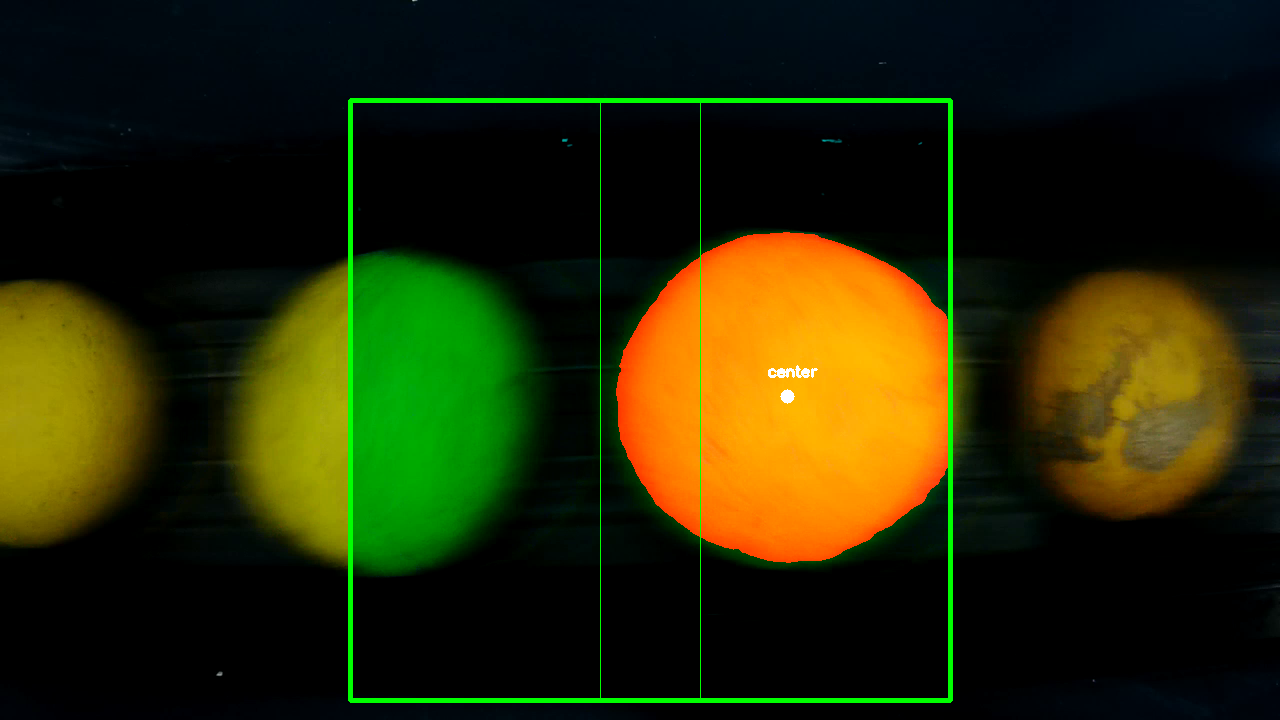
\includegraphics[width=0.45\linewidth]{2023_ConteoNaranjasBandaTransportadora/figs/framito.png} &
		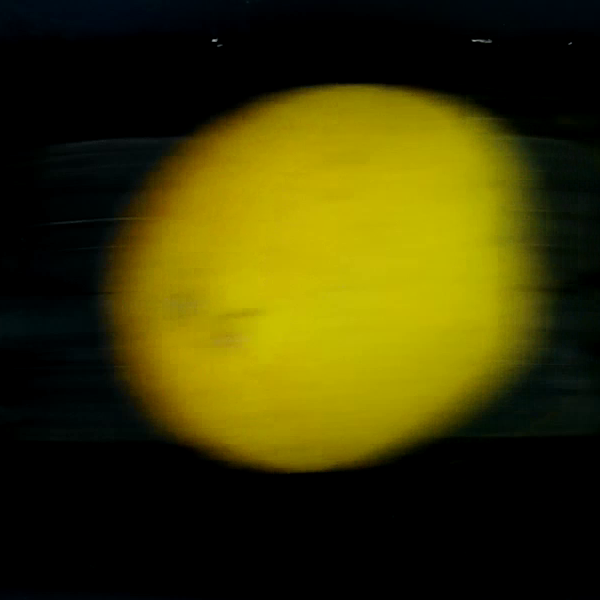
\includegraphics[width=0.25\linewidth]{2023_ConteoNaranjasBandaTransportadora/figs/blur.png} &
		
\includegraphics[width=0.25\linewidth]{2023_ConteoNaranjasBandaTransportadora/figs/blurmask.png} \\
	\end{tabular}
\end{center}
\end{frame}


\begin{frame}{\citetitle{\EntradaBibtex} (5)}
\begin{itemize}
\item Es posible obtener precisiones de 94\% con respecto al color y 96\% con respecto al tamaño 
\item El sistema ya acoplado con la banda transportadora puede clasificar hasta 5 naranjas por segundo (3.6 toneladas por hora)
\item La principal limitante de la velocidad de clasificación son los elementos mecánicos (banda transportadora, actuadores, etc). El sistema de visión en teoría puede procesar 60 naranjas por segundo (43.2 toneladas por hora)
\end{itemize}

\end{frame}


